\documentclass[12pt]{article}
\usepackage{amsmath}
\usepackage{array}
% \usepackage{gensymb}
\usepackage{geometry}
\usepackage{graphicx}
\usepackage{pgfplots}
\usepackage{siunitx}
\usepackage{wrapfig}

\title{Homework \#16}
\author{Donald Aingworth IV}
\date{December 11, 2024}

\pgfplotsset{width=8cm,compat=1.9}
\usepgfplotslibrary{external}
% \tikzexternalize

\begin{document}

\DeclareSIUnit{\mile}{mi}
\DeclareSIUnit{\gal}{gal}
\DeclareSIUnit{\foot}{ft}
\DeclareSIUnit{\hour}{h}
\DeclareSIUnit{\rad}{rad}
\DeclareSIUnit{\unit}{u}
\DeclareSIUnit{\dyne}{dyn}

\maketitle

\pagebreak
\section{Problem 1}
Two disks are mounted (like a merry-go-round) on low-friction bearings on the same axle and can be brought together so that they couple and rotate as one unit. The first disk, with rotational inertia 3.30 \unit{\kilo\gram*\meter^2} about its central axis, is set spinning counterclockwise at 450 rev/min. The second disk, with rotational inertia 6.60 \unit{\kilo\gram*\meter^2} about its central axis, is set spinning counterclockwise at 900 rev/min. They then couple together. (a) What is their angular speed after coupling? If instead the second disk is set spinning clockwise at 900 rev/min, what are their (b) angular speed and (c) direction of rotation after they couple together?

\subsection{Solution}
\subsubsection{Section (a)}
We have a concept called conservation of angular momentum. 
\begin{align}
    L_i &=  L_f\\
    L_f &=  l_1 + l_2
        =   I_1\omega_1 + I_2\omega_2\\
    \omega_f    &=  \frac{I_1\omega_1 + I_2\omega_2}{I_1 + I_2}
        =   \frac{3.3*450 + 6.6*900}{3.3 + 6.6}\\
        &=  \frac{1485 + 5940}{9.9}
        =   \boxed{750\text{rev/min}}
\end{align}

\subsubsection{Section (b)}
We just need to change a positive to a negative. 
\begin{align}
    \omega_f    &=  \frac{I_1\omega_1 + I_2\omega_2}{I_1 + I_2}
        =   \frac{3.3*450 - 6.6*900}{3.3 + 6.6}\\
        &=  \frac{1485 - 5940}{9.9}
        =   -450\text{rev/min}\\
    |\omega_f|  &=  \boxed{450\text{rev/min}}
\end{align}

\subsubsection{Section (c)}
Since the value is negative and negative angular velocity corresponds to clockwise motion, the angular motion is \boxed{clockwise}.

\pagebreak
\section{Problem 2}
The Sun's mass is 2.0 \texttimes $10^{30}$ kg, its radius is 7.0 \texttimes $10^5$ km, and it has a rotational period of approximately 28 days. If the Sun should collapse into a white dwarf of radius 3.5 \texttimes $10^3$ km, what would its period be if no mass were ejected and a sphere of uniform density can model the Sun both before and after?

\subsection{Solution}
% We first find the moment of inertia of the sun, which is a solid sphere rotating about its diameter, so the formula is \( I = \frac{2}{5}MR^2 \). 
% \begin{align}
%     I   &=  \frac{2}{5}MR^2
%         =   \frac{2}{5} * (2.0 \times 10^{30}) * (7.0 \times 10^{5})^2
%         =   \frac{2}{5} * (2.0 \times 10^{30}) * (49.0 \times 10^{10})\\
%         &=  \frac{1}{5} * (98.0 \times 10^{40})
%         =   19.6 \times 10^{40} \unit{\kilo\gram*\meter^2}
% \end{align}

We can calculate the angular frequency of the sun by using the period formula \(T = \frac{2\pi}{\omega}\).
\begin{align}
    T   &=  \frac{2\pi}{\omega}\\
    \omega  &=  \frac{2\pi}{T}
\end{align}

Next, we can use the conservation of angular momentum and the formula for the inertia of the dwarf sun to find a formula for the final angular velocity and then final period.
\begin{align}
    L_f &=  L_i\\
    I_f\omega_f &=  I_i\omega_i\\
    I_f\frac{2\pi}{T_f} &=  I_i\frac{2\pi}{T_i}\\
    \frac{I_f}{I_i}\cdot\frac{2\pi}{2\pi}   &=  \frac{T_f}{T_i}\\
    \frac{I_f}{I_i}*T_i &=  T_f\\
    \frac{\frac{2}{5}MR_f^2}{\frac{2}{5}MR_i^2}*T_i =
    \frac{R_f^2}{R_i^2}*T_i =
    \frac{(3.5 \times 10^{3})^2}{(7.0 \times 10^{5})^2}*28\text{days}   &=  T_f\\
    \frac{12.25 \times 10^{6}}{49.0 \times 10^{10}}*28\text{days}   =
    \frac{28\text{days}}{4 \times 10^4} =
    7 \times 10^{-4} \text{days}    &=  T_f
\end{align}

This means that the period is \boxed{7 \times 10^{-4} \text{ days}}.
\pagebreak
\section{Problem 3}
The displacement from equilibrium of a particle is given by \(x(t) = A \cos\left(\omega t - \frac{\pi}{3}\right)\). Which, if any, of the following are equivalent expressions:
\begin{align}
    a)\ x(t)    &=  A\cos\left(\omega t + \frac{\pi}{3}\right)\\
    b)\ x(t)    &=  A\cos\left(\omega t + \frac{5\pi}{3}\right)\\
    c)\ x(t)    &=  A\cos\left(\omega t + \frac{\pi}{6}\right)\\
    d)\ x(t)    &=  A\cos\left(\omega t - \frac{5\pi}{6}\right)
\end{align}

\subsection{Solution}
We can see that the only change here is the part labeled $\phi$ in the format of simple harmonic motion. For an equivalent value, the value of the cosine must be the same at every point, which can only be true if \(\phi = -\frac{\pi}{3} \mod 2\pi\).

\begin{tabular}{c | c | c | c}
        &   $\phi$  &   $\phi\mod 2\pi$ &   Correct?\\ \hline
        &   $-\frac{\pi}{3}$    &   $\frac{5\pi}{3}$    &   Yes\\
    a)  &   $\frac{\pi}{3}$     &   $\frac{\pi}{3}$     &   No\\
    b)  &   $\frac{5\pi}{3}$    &   $\frac{5\pi}{3}$    &   Yes\\
    c)  &   $\frac{\pi}{6}$     &   $\frac{\pi}{6}$     &   No\\
    d)  &   $\frac{5\pi}{6}$    &   $\frac{5\pi}{6}$    &   No
\end{tabular}

\pagebreak
\section{Problem 4}
In a block and spring system $m = 0.250 \unit{\kilo\gram}$ and $k = 4.00 \unit{\newton/\meter}$. At $t = 0.150 \unit{\second}$, the velocity is $v = -0.174 \unit{\meter/\second}$ and the acceleration $a = +0.877 \unit{\meter/\second^2}$. Write an expression for the displacement as a function of time, $x(t)$. (Hint, remember that the inverse tan function only returns the principal value, but there is a secondary value as well.)

\subsection{Solution}
We have some formulas for velocity and acceleration that we can use.
\begin{align}
    \omega  &=  \sqrt{\frac{k}{m}}
        =   \sqrt{\frac{4.0}{0.25}} =   \sqrt{4^2}
        =   4\unit{\second^{-1}}\\
    v(t)    &=  -\omega x_m \sin(\omega t + \phi)\ \ \rightarrow
    v(0.15) =   -0.174 \unit{\meter/\second}
        =   -4 x_m \sin(0.6 + \phi)\\
    a(t)    &=  -\omega^2 x_m \cos(\omega t + \phi)\rightarrow
    a(0.15) =   \ 0.877 \unit{\meter/\second^2}
        =   -16 x_m \cos(0.6 + \phi)\\
    \frac{a(0.15)}{v(0.15)} &=  \frac{-16 x_m \cos(0.6 + \phi)}{-4 x_m \sin(0.6 + \phi)}
        =   4*\frac{\cos(0.6 + \phi)}{\sin(0.6 + \phi)}\\
    \tan(\phi)  &=  \frac{\sin(\phi)}{\cos(\phi)}
        =   \frac{v(0)\sqrt{k}}{a(0)\sqrt{m}}\\
    0.6 + \phi  &=  \arctan\left(4*\frac{v(0)}{a(0)}\right)
        =   \arctan\left(4*\frac{-0.174}{0.877}\right)\\
        &=  \arctan\left(-\frac{0.696}{0.877}\right)
        =   \begin{matrix} 2.471 \\ 5.612 \end{matrix}
\end{align}

One of these is in the second quadrant, the other is in the fourth quadrant. Knowing that $\omega$ is positive and trusting that $x_m$ is positive, since the negative cosine is positive and the negative sine is negative, the cosine is negative and the sine is positive, so $0.6 + \phi$ is in the second quadrant. This means $0.6 + \phi = 2.471$ and $\phi = 1.871$. Last, we just neeed to find the value of $x_m$, which we will find using the value of $a(0)$.
\begin{align}
    a(0.15)    &=  -16 x_m \cos(0.6 + 1.871)\\
    x_m &=  -\frac{a(0)}{16\cos(2.471)}
        =   \frac{0.877}{0.7833}
        =   0.06998\unit{\meter}
\end{align}

Lastly, we find the value of $\omega$ and use that to finalize the formula for $x(t)$. 
\begin{equation}
    \boxed{x(t) =  0.06998*\cos(4t + 1.871)}
\end{equation}

\pagebreak
\section{Problem 5}
A 60.0 g block attached to a horizontal spring is held at 8.00 cm from its equilibrium position and released at $t = 0$. Its period is $0.900 \unit{\second}$. Find: (a) the displacement $x$ at $1.20 \unit{\second}$; (b) the velocity when $x = -5.00 \unit{\centi\meter}$; (c) the acceleration when $x = -5.00 \unit{\centi\meter}$; (d) the total energy.

\subsection{Solution}
\subsubsection{Section (a)}
To find the position, we can use the simple harmonic motion formula. We can set $x_m = 8.0\unit{\centi\meter}$. Next, we need to find $\omega$. Since it starts from the fullest extension at $t = 0$, $\phi = 0$.
\begin{align}
    \omega  &=  \frac{2\pi}{T}\\
    x(t)    &=  x_m \cos(\omega t + \phi)
        =   x_m \cos\left( \frac{2\pi}{T}t + \phi \right)\\
        &=  8.0 * \cos\left( \frac{2\pi}{0.900}t \right)\\
    x(1.2)  &=  8.0 * \cos\left( \frac{2\pi}{0.900}*1.2 \right)
        =   8.0 * \cos\left( \frac{24\pi}{9} \right)\\
        &=  8.0 * \cos\left( \frac{8\pi}{3} \right)
        =   8.0 * (-0.5)
        =   -4.0\unit{\centi\meter}
\end{align}
This means that the block is \boxed{4 \unit{\centi\meter}} away from the equilibrium.

\subsubsection{Section (b)}
First, we find the time at whch $x = 5.00\unit{\centi\meter}$.
\begin{gather}
    -5\unit{\centi\meter}   =   8.0 * \cos\left( \frac{2\pi}{0.900}t \right)\\
    \cos\left(\frac{2\pi}{0.900}t\right) =   -\frac{5}{8}
\end{gather}

By using the pythagorean theorem, we can find a value for $\sin\left(\frac{2\pi}{0.900}t\right)$.
\begin{gather}
    \sin^2(\theta)  =   1 - \cos^2(\theta)\\
    \sin(\theta)    =   \sqrt{1 - \cos^2(\theta)}\\
    \sin\left(\frac{2\pi}{0.900}t\right)    =   \sqrt{1 - \cos^2\left(\frac{2\pi}{0.900}t\right)}\\
    \sin\left(\frac{2\pi}{0.900}t\right)    =   \sqrt{1 - \frac{5}{8}^2} = \frac{\sqrt{39}}{8}
\end{gather}

The SHM velocity is the first derivatve of the SHM position.
\begin{align}
    x(t)    &=  8.0 * \cos\left( \frac{2\pi}{0.900}t \right)\\
    \frac{dx(t)}{dt}    =
    v(t)    &=  -8.0 * \frac{2\pi}{0.900} * \sin\left( \frac{2\pi}{0.900}t \right)
        =   -\frac{16\pi}{0.900} * \sin\left( \frac{2\pi}{0.900}t \right)\\
    v(t_1)  &=  -\frac{16\pi}{0.900}*\frac{\sqrt{39}}{8}
        =   -\frac{20\pi\sqrt{39}}{9}
        =   -43.598\unit{\centi\meter/\second}
\end{align}
This means that the velocity is \boxed{43.598\unit{\meter/\second}}.

\subsubsection{Section (c)}
From our in-class differential equations for SHM, we know that \(\frac{d^2 x(t)}{dt^2} = -\omega^2 x(t)\). We can work with this, recalling that $\omega = \frac{2\pi}{T}$.
\begin{align*}
    \frac{d^2 x(t)}{dt^2}   &=  a(t)
        =   -\omega^2 x(t)
        =   \left(\frac{2\pi}{T}\right)^2 * x(t)\\
    a   &=  \frac{4\pi^2}{T^2} * x
        =   \frac{4\pi^2}{0.9^2} * 5
        =   \boxed{243.694\unit{\centi\meter/\second^2}}
\end{align*}

\subsubsection{Section (d)}
We can calculate this using the velocity where there is no potential energy (where x = 0). This can only be true where $cos(\theta) = 0$, since the equivalent of $\theta$ is the only variable without a set value (yet). With the pythagorean theorem, if $cos(\theta) = 0$, $\sin(\theta) = \pm 1$, with either one working, so we will be using $-1$.
\begin{gather}
    v   =   -\frac{16\pi}{0.900} * \sin\left( \frac{2\pi}{0.900}t \right)
        =   -\frac{16\pi}{0.900} * (-1)
        =   \frac{16\pi}{0.900}\unit{\centi\meter/\second}
\end{gather}\begin{align}
    E_{total}   &=  K + U
        =   \frac{1}{2}mv^2 + \frac{1}{2}kx^2
        =   \frac{1}{2}*(60.0\unit{\gram})*\left(\frac{16\pi}{0.900}\unit{\centi\meter/\second}\right)^2 + 0\\
        &=  \boxed{93578\ \unit{\dyne*\centi\meter} = 9.3578\times10^{-3}\unit{\joule}}
\end{align}


\pagebreak
\section{Problem 6}
\begin{wrapfigure}{r}{0.15\textwidth}
    \vspace{-30pt}
    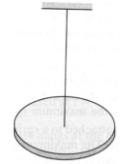
\includegraphics[width=0.15\textwidth]{graph_6.png} 
    % \label{fig:wrapfig}
\end{wrapfigure}
A wire has a torsional constant $\kappa = 2.00 \unit{\newton*\meter/\rad}$. A solid disk of radius $R = 5.00 \unit{\centi\meter}$ and mass $M = 100 \unit{\gram}$ is suspended at its center as shown in the figure. What is the frequency of torsional oscillations?

\subsection{Solution}
First, I want to convert the whole thing to the SI unit system, so the radius is $0.05 \unit{\meter}$ and the mass is $0.1 \unit{\kilo\gram}$. The frequency is equal to the reciprocal of the period, and we have a formula for the period.
\begin{align}
    T   &=  \frac{1}{f}
        =   2\pi\sqrt{\frac{I}{\kappa}}\\
    f   &=  \frac{1}{T}
        =   \frac{1}{2\pi}\sqrt{\frac{\kappa}{I}}\\
        &=  \frac{1}{2\pi}\sqrt{\frac{2\kappa}{MR^2}}
        =   \frac{1}{2\pi}\sqrt{\frac{2*2}{0.1*0.05^2}}\\
        &=  \frac{1}{2\pi}\sqrt{\frac{4}{2.5\times10^{-4}}}
        =   \frac{1}{\pi\sqrt{2.5\times10^{-4}}}\\
        &=  \boxed{20.13 \unit{\hertz}}
\end{align}

\pagebreak
\section{Problem 7}
The total energy of a block and spring system is $0.200 \unit{\joule}$. The mass of the block is $120 \unit{\gram}$ and the spring constant is $40 \unit{\newton/\meter}$. Find: (a) the amplitude; (b) the maximum speed; (c) the displacement from equilibrium when the speed is $1.30 \unit{\meter/\second}$; (d) the maximum acceleration.

\subsection{Solution}
\subsubsection{Section (a)}
When there is no velocity (and the sine value is zero), the cosine value is one. All the energy would also be spring potential energy. 
\begin{align}
    x   &=  x_{m}\cos(\omega t + \phi)
        =   x_{m}\\
    0.200   &=  \frac{1}{2}kx^2\\
    0.400   &=  40*x^2\\
    0.01    &=  x^2\\
    x   &=  \boxed{x_m
        =   0.1\unit{\meter}}
        =   \sqrt{0.01}
\end{align}

\subsubsection{Section (b)}
The maximum speed will be achieved when all the energy is kinetic.
\begin{align}
    0.200   &=  \frac{1}{2}mv^2\\
    v^2 &=  \frac{0.400}{0.12}\\
    v   &=  \sqrt{\frac{10}{3}}
        =   \frac{\sqrt{30}}{3}
        =   \boxed{1.8257\unit{\meter/\second}}
\end{align}

\subsubsection{Section (c)}
We can plug in values into the energy and isolate the postional value.
\begin{align}
    E   &=  K + U
        =   \frac{1}{2}mv^2 + \frac{1}{2}kx^2\\
    kx^2    &=  2E - mv^2\\
    x   &=  \sqrt{\frac{2E - mv^2}{k}}
        =   \sqrt{\frac{2*0.200 - 0.12*1.3^2}{40}}
        =   \sqrt{\frac{0.4 - 0.2028}{40}}\\
        &=  \sqrt{\frac{0.1972}{40}}
        =   \sqrt{4.93\times10^{-3}}
        =   \boxed{0.07021\unit{\meter}}
\end{align}

\subsubsection{Section (d)}
We can use our differential equation to find this, given our maximum position and an unchanging $\omega$.
\begin{align}
    \frac{d^2 x(t)}{dt^2}   &=  a(t)
        =   -\omega^2 x(t)
        =   -\frac{k}{m} * x(t)\\
    |a| &=  \frac{k}{m} * x
        =   \frac{40}{0.12} * 0.1
        =   \boxed{\frac{100}{3}\unit{\meter/\second^2}
        =   33.33\unit{\meter/\second^2}}
\end{align}

\pagebreak
\section{Problem 8}
A uniform rod of mass $M$ and length $L = 1.20 \unit{\meter}$ oscillates about a horizontal axis at one end. What is the length of the simple pendulum that would have the same period? The rotational inertia is $\frac{ML^2}{3}$.

\subsection{Solution}
What we have here is a physical pendulum, and we want to compare it to a simple pendulum. We can create an equality. Since we know that the two values are equal, we don't have separate kinds of the variable T. 
\begin{gather}
    T   =   2\pi\sqrt{\frac{L_s}{g}}\\
    T   =   2\pi\sqrt{\frac{I}{mgh}}
        =   2\pi\sqrt{\frac{ML_p^2}{3Mgh}}
\end{gather}
To be clear, the first eqution is for a simple equation, while the second is for a physical pendulum.

\begin{align}
    I   &=  \frac{1}{3}ML^2\\
    2\pi\sqrt{\frac{L_s}{g}}    &=  2\pi\sqrt{\frac{ML_p^2}{3Mgh}}\\
    \sqrt{\frac{L_s}{g}}  &=  \sqrt{\frac{L_p^2}{3gh}}\\
    \frac{L_s}{g}   &=  \frac{L_p^2}{3gh}\\
    L_s &=  \frac{L_p^2}{3h}
\end{align}

To conclude this, we can know that the center of mass ($h$) of the uniform rod pendulum is going to be \(h = \frac{L_p}{2}\).
\begin{equation}
    L_s =   \frac{L_p^2}{3h}
        =   \frac{2L_p^2}{3h}
        =   \frac{2}{3}L_p
        =   \frac{2}{3}*1.20\unit{\meter}
        =   \boxed{0.8\unit{\meter}}
\end{equation}


\end{document}